% =====================================================================
%  A1 PORTRAIT POSTER TEMPLATE (594 x 841 mm)
%  Topic: RGB-D topological mapping / two-layer GNG for the ceiling robot
%
%  This is a CLONE of docs/poster_A1_energy_aware/poster_energy_aware_A1.tex:
%  identical layout, colours and macros, but the content is a skeleton.
%
%  >>> HOW TO USE <<<
%   1. Everything wrapped in \TODO{...} is a placeholder -- it prints in RED
%      so an unfinished poster is obvious. Replace, do not just delete the
%      macro, or the surrounding sentence may stop making sense.
%   2. \FIGBOX{<height>}{<caption>} is a grey placeholder frame. Swap it for
%      \IG{<width fraction>}{<file in figure/>} once the real asset exists.
%   3. NEVER type a number you have not measured. Leave it as \TODO{}.
%   4. Section text below is drawn from the reachability_gng README (method,
%      not results), so the *how it works* parts are already accurate.
%
%  Build:  pdflatex poster_rgbd_topo_A1.tex
%
%  Tuning knobs (preamble): \bodysize / \bodyskip for all body text,
%  \pillsize for section headers, \figscale scales every \IG figure.
% =====================================================================
\documentclass[20pt,a4paper]{extarticle}

\usepackage[
  paperwidth=594mm, paperheight=841mm,
  left=14mm, right=14mm, top=13mm, bottom=13mm
]{geometry}

\usepackage[T1]{fontenc}
\usepackage[utf8]{inputenc}
\usepackage[scaled=0.98]{helvet}
\renewcommand{\familydefault}{\sfdefault}

\usepackage{amsmath,amssymb}
\usepackage{graphicx}
\usepackage{xcolor}
\usepackage[most]{tcolorbox}
\usepackage{tikz}
\usetikzlibrary{positioning,calc,arrows.meta}
\usepackage{eso-pic}
\usepackage{enumitem}
\usepackage{booktabs}
\usepackage{array}
\usepackage{ragged2e}
\usepackage{anyfontsize}

\graphicspath{{figure/}}

% ------------------------------------------------------------- knobs
\newcommand{\bodysize}{17}
\newcommand{\bodyskip}{21}
\newcommand{\pillsize}{25}
\def\figscale{0.95}
\newcommand{\IG}[2]{\includegraphics[width=\figscale\dimexpr#1\linewidth\relax]{#2}}

% ---------------------------------------------------------------- colors
\definecolor{pgold}{HTML}{F5B335}
\definecolor{pgoldd}{HTML}{D98C0F}
\definecolor{pbody}{HTML}{1A1A1A}
\definecolor{pblue}{HTML}{1F4E79}
\definecolor{pgrey}{HTML}{6E6E6E}

\color{pbody}
\setlength{\parindent}{0pt}
\setlength{\parskip}{3pt}
\renewcommand{\arraystretch}{1.12}

% ------------------------------------------------- outer rounded frame
\AddToShipoutPictureBG{%
  \begin{tikzpicture}[remember picture, overlay]
    \draw[pgold, line width=3.2pt, rounded corners=16pt]
      ($(current page.south west)+(8mm,8mm)$)
      rectangle
      ($(current page.north east)+(-8mm,-8mm)$);
  \end{tikzpicture}%
}

% ------------------------------------------------------ section pill
\newtcolorbox{sectionpill}{
  enhanced, width=\linewidth,
  colback=pgold, colframe=pgold,
  arc=8mm, boxrule=0pt,
  left=4mm, right=4mm, top=1.2mm, bottom=1.2mm,
  halign=flush center, valign=center,
  before skip=5mm, after skip=2.5mm
}
\newcommand{\psection}[1]{%
  \begin{sectionpill}\bfseries\fontsize{\pillsize}{\pillsize}\selectfont #1\end{sectionpill}}

% ------------------------------------------------------ highlight box
\newtcolorbox{keybox}{
  enhanced, width=\linewidth,
  colback=pgold!16!white, colframe=pgold,
  arc=4mm, boxrule=1.4pt,
  left=4mm, right=4mm, top=2.5mm, bottom=2.5mm,
  before skip=3mm, after skip=3mm
}

% ------------------------------------------------------ list styles
\setlist[itemize,1]{leftmargin=6.5mm, topsep=1pt, itemsep=2pt,
                    parsep=0pt, label=\textcolor{pgoldd}{$\bullet$}}
\setlist[itemize,2]{leftmargin=6mm, topsep=1pt, itemsep=1pt,
                    parsep=0pt, label=\textcolor{pgoldd}{$\circ$}}

% ------------------------------------------------------ helpers
\newcommand{\figcap}[1]{{\par\vspace{0.8mm}\centering
  \fontsize{14}{17}\selectfont\itshape\color{pgrey}#1\par\vspace{0.8mm}}}
\newcommand{\num}[1]{\textcolor{pblue}{\bfseries #1}}
\newcommand{\lead}[1]{\textbf{#1}}

% -------------------------------------------- placeholders (REMOVE LATER)
\newcommand{\TODO}[1]{\textcolor{red}{\bfseries[TODO: #1]}}
\newcommand{\FIGBOX}[2]{%
  \begin{center}
  \begin{tcolorbox}[enhanced, width=\linewidth, height=#1,
    colback=pgrey!8!white, colframe=pgrey!45!white, boxrule=1.2pt,
    arc=3mm, halign=center, valign=center, before skip=2mm, after skip=1mm]
    {\fontsize{16}{19}\selectfont\color{pgrey}\itshape figure placeholder\\[1mm]#2}
  \end{tcolorbox}
  \end{center}}

\pagestyle{empty}

\begin{document}
\fontsize{\bodysize}{\bodyskip}\selectfont

% =====================================================================
%  HEADER
% =====================================================================
\begin{tcolorbox}[enhanced, width=\linewidth,
  colback=white, colframe=pgold, arc=10mm, boxrule=2.6pt,
  left=6mm, right=6mm, top=2mm, bottom=2mm]
\begin{minipage}[c]{0.085\linewidth}
  \centering
  \bfseries\fontsize{34}{34}\selectfont P-XX
\end{minipage}%
\begin{minipage}[c]{0.79\linewidth}
  \centering
  {\bfseries\fontsize{18}{21}\selectfont
   2026 The Term-End Evaluation, Department of Mechanical Systems Engineering, TMU.\par}
  \vspace{2mm}
  {\bfseries\fontsize{36}{42}\selectfont
   \TODO{poster title, line 1}\\
   \TODO{poster title, line 2}\par}
  \vspace{2.5mm}
  {\bfseries\fontsize{22}{26}\selectfont
   Naoyuki Kubota Laboratory, D2, Raditya Artha Rochmanto\par}
  {\fontsize{18}{22}\selectfont
   email: rochmanto-artha@ed.tmu.ac.jp\par}
\end{minipage}%
\begin{minipage}[c]{0.125\linewidth}
  \centering
  
\includegraphics[width=1\linewidth]{tmu_logo.jpg}\\[1.5mm]
  {\bfseries\fontsize{14}{16}\selectfont\color{pgrey} CONFIDENTIAL}
\end{minipage}
\end{tcolorbox}

% ------------------------------------------------------------- tagline
\begin{center}
  \bfseries\fontsize{23}{27}\selectfont
  \TODO{one-sentence claim of the poster, first half}\\
  \TODO{second half --- keep it to two lines}
\end{center}

\vspace{-1mm}

% =====================================================================
%  TWO COLUMNS
% =====================================================================
\noindent
\begin{minipage}[t]{0.487\linewidth}
% ================================================= LEFT COLUMN =======

\psection{Background}

\begin{minipage}[t]{0.40\linewidth}
  \vspace{0pt}
  \FIGBOX{62mm}{workspace / robot photo}
\end{minipage}\hfill
\begin{minipage}[t]{0.57\linewidth}
  \vspace{0pt}\RaggedRight
  \TODO{2--3 sentences: why a ceiling robot in a home, and why it needs a map
  of its surroundings rather than a raw point cloud.}
\end{minipage}

\vspace{1.5mm}
\lead{Platform.} Two ceiling rails (gantries), two Kinova Gen3 Lite arms each,
so every arm is an \textbf{8-DOF} chain $\mathbf{q}=[d,\theta,q_1\ldots q_6]$
sharing one moving base with its neighbour. Sensing is \textbf{RGB-D only} ---
no LIDAR.

\psection{Problems}

\begin{itemize}
  \item \lead{P1 --- \TODO{name the first problem}.} \TODO{one or two lines.}
  \item \lead{P2 --- A raw octomap has no structure.} Occupancy alone gives no
        topology: no notion of which regions connect, and every frame is paid
        for again.
  \item \lead{P3 --- Static and dynamic obstacles are mixed.} With a single
        live map, the fixed structure of the room and a person walking through
        it are indistinguishable, so the map is never reproducible between runs.
\end{itemize}

\psection{RGB-D Sensing and Extrinsic Calibration}

\begin{itemize}
  \item Two overhead RGB-D cameras are the \emph{only} exteroceptive sensor;
        their extrinsics are recovered with a \textbf{ChArUco} board and
        published as \texttt{world}\,$\rightarrow$\,camera static transforms.
  \item \texttt{depth\_cloud} deprojects each depth image into world-frame
        points \textbf{without any segmentation gate}, so the map keeps building
        even when the detector is blind.
  \item \TODO{calibration residual / reprojection error, once measured.}
\end{itemize}

\FIGBOX{55mm}{ChArUco calibration + the two camera views}

\psection{Two-Layer Topological Map (GNG)}

\begin{itemize}
  \item A \textbf{Growing Neural Gas} network is fitted to the live depth cloud:
        nodes tile the observed geometry and competitive Hebbian edges give the
        scene a \emph{topology}, not just occupancy.
  \item \lead{Static layer} --- captured once on a cleared scene and frozen to a
        file, giving a backbone that is \emph{identical every run}.
  \item \lead{Dynamic layer} --- live points within \texttt{bg\_dist} of a static
        node are subtracted, so the live map carries only the genuinely moving
        remainder (a person, a displaced object).
  \item Both layers are unioned into the planning scene, so MoveIt~2 plans
        against fixed structure and dynamic obstacles at once.
\end{itemize}

\FIGBOX{60mm}{RViz: blue static backbone vs.\ green dynamic remainder}

\end{minipage}\hfill
% ================================================= RIGHT COLUMN ======
\begin{minipage}[t]{0.487\linewidth}

\psection{Pipeline}

{\centering
\resizebox{\linewidth}{!}{%
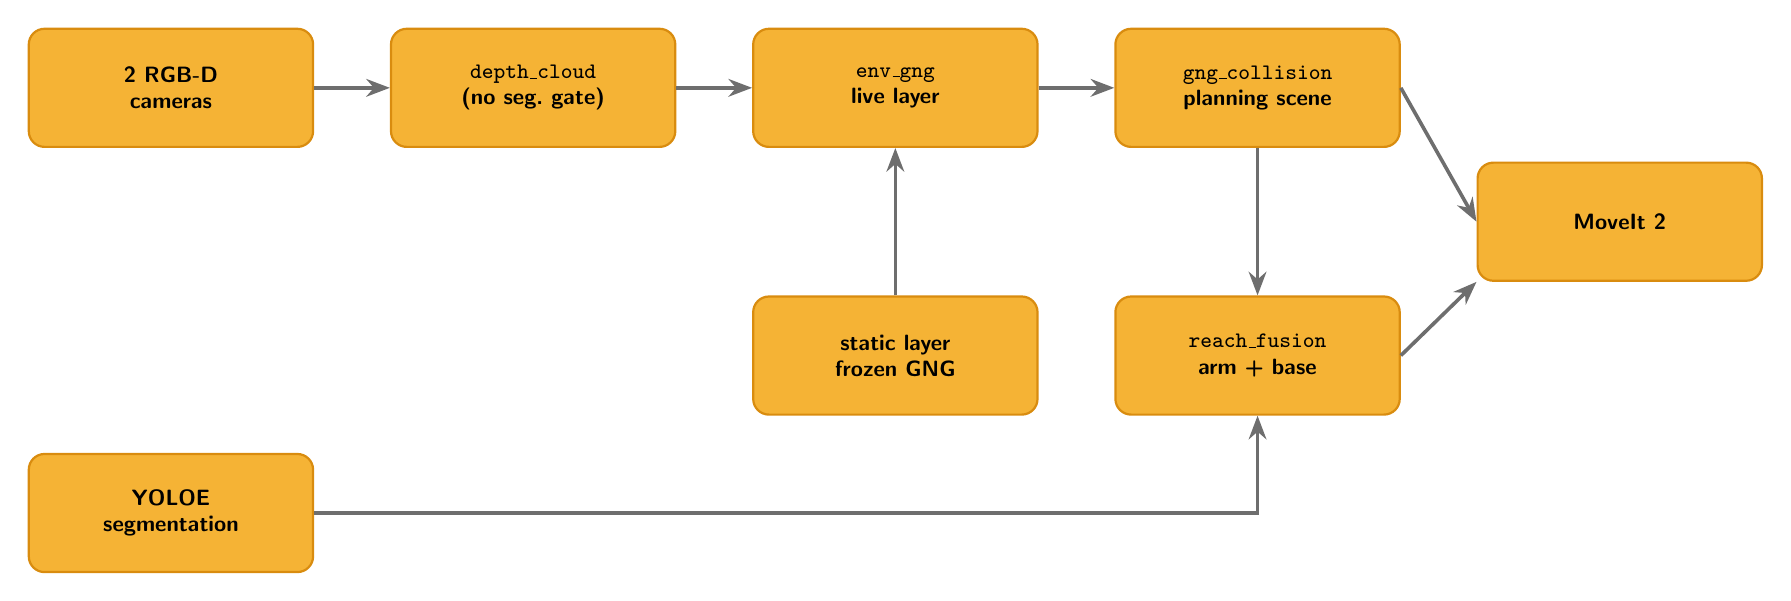
\begin{tikzpicture}[>=Stealth, thick, font=\footnotesize,
  box/.style={draw=pgoldd, fill=pgold, text=black, rounded corners=2mm,
              align=center, minimum height=15mm, text width=34mm, inner sep=3pt,
              font=\bfseries\footnotesize},
  arr/.style={-{Stealth[length=3mm]}, line width=1.3pt, draw=pgrey}]
  % --- geometry path (top row)
  \node[box] (cam) at (0,0)      {2 RGB-D\\cameras};
  \node[box] (dc)  at (4.6,0)    {\texttt{depth\_cloud}\\(no seg.\ gate)};
  \node[box] (gng) at (9.2,0)    {\texttt{env\_gng}\\live layer};
  \node[box] (col) at (13.8,0)   {\texttt{gng\_collision}\\planning scene};
  % --- static layer feeding the live map from below
  \node[box] (stat) at (9.2,-3.4) {static layer\\frozen GNG};
  % --- identity path (bottom row)
  \node[box] (seg) at (0,-5.4)   {YOLOE\\segmentation};
  \node[box] (fus) at (13.8,-3.4) {\texttt{reach\_fusion}\\arm + base};
  \node[box] (mv)  at (18.4,-1.7) {MoveIt~2};
  \draw[arr] (cam)  -- (dc);
  \draw[arr] (dc)   -- (gng);
  \draw[arr] (gng)  -- (col);
  \draw[arr] (stat) -- (gng);
  \draw[arr] (col)  -- (fus);
  \draw[arr] (seg)  -| (fus.south);
  \draw[arr] (col.east) -- (mv.west);
  \draw[arr] (fus.east) -- (mv.south west);
\end{tikzpicture}}\par}
\figcap{Geometry (top path) is decoupled from identity (bottom path): the
topological map builds from \texttt{depth\_cloud} alone, so it survives a
detector that sees nothing.}

\psection{Object Identity and Tracking}

\begin{itemize}
  \item Detections are associated across frames by \textbf{Hungarian matching}
        with a distance gate and a class-consistency cost, so an object keeps
        one stable track handle.
  \item A track is only published after an \textbf{N-frame confirmation}, and
        its class label is decided by \textbf{majority voting with hysteresis},
        which removes the frame-to-frame label flipping.
  \item Safety is \textbf{geometry-based}: the collision map does not depend on
        labels, and only the confirmed target is carved out of it.
  \item \TODO{state which detector the final results use (YOLOE or the
        simulator's ground-truth segmentation) and why.}
\end{itemize}

\psection{Experiments}

\lead{E\TODO{n} --- \TODO{experiment name}.} \TODO{one sentence on the setup:
what was varied, how many trials, what was measured.}

\vspace{1mm}
{\centering\fontsize{16}{20}\selectfont
\begin{tabular}{@{}l c c c@{}}
\toprule
\textbf{Condition} & \textbf{\TODO{metric 1}} & \textbf{\TODO{metric 2}} & \textbf{\TODO{metric 3}}\\
\midrule
\TODO{baseline} & --- & --- & ---\\
\TODO{ours}     & --- & --- & ---\\
\bottomrule
\end{tabular}\par}
\figcap{\TODO{table caption: state the sample size and what "---" will become.}}

\FIGBOX{62mm}{results plot}

\begin{keybox}
\TODO{the single headline result, with its number and its honest caveat ---
write it only once it is measured.}
\end{keybox}

\psection{Summary and Contributions}

\begin{keybox}
\begin{itemize}[leftmargin=6mm, topsep=0pt]
  \item \TODO{contribution 1 --- the representation.}
  \item \TODO{contribution 2 --- the static/dynamic split.}
  \item \TODO{contribution 3 --- what the evaluation shows.}
\end{itemize}
\end{keybox}

\lead{Future work.} \TODO{one or two sentences.}

\end{minipage}

\vspace{3mm}
{\fontsize{13}{15.5}\selectfont\color{pgrey}
\textbf{References.}
[1]~Fritzke, NIPS 1995 (GNG).
[2]~\TODO{add the references this poster actually cites, in the order they are
cited above; keep the bracket numbers consistent with the body text.}
\par}

\end{document}
